%TODO introduction to software implementation. C programming language, pthreads, webserver.
The software has been implemented in the C programming language to allow for maximum re-use of components across the master unit (Raspberry Pi, Linux) and the scale units (STM32F4/ARM Cortex M4 microcontroller, no operating system). These Units are connected to each other through a ``star'' network topology using the ZigBee RF modules. One ZigBee, connected to the master unit, is configured as a coordinator (ie. access point) and the four others as routers (or end devices). They join the network with a pre-set network ID and can then communicate wirelessly. To avoid having to store and discover network addresses, only broadcast mode (coordinator to all other devices) and unicast to the coordinator (since the coordinator adress does never change) are used.

%overview
\section{Packet Protocol}
\label{section:software-impl-packets}
ZigBee modules can operate in two seperate communication modes. Firstly, transparent mode is the most basic one, where only very simple packetization (after a time-out or when a buffer is filled) is provided. In this mode it is very simple to set up a basic point-to-point network, but it does not support multiple nodes transmitting at once. In that situation, packets can become interleaved, rendering this mode not very useful for the envisioned star network architecture. Still, it proved useful for initial debugging and manually sending data by connecting the device directly to a serial terminal.

The second mode supported is the ZigBee API, where data is not immediately transmitted, but a series of command packets must be sent to the ZigBee device over the serial connection in order to request data transmission. Here, the ZigBee layer guarantees delivery (up to \textbf{TODO check this number with data sheet and cite} 3 retransmissions) and maintains packet boundaries. The API defines a wrapper packet protocol that is used for sending command and data frames across the serial link\cite[page 35]{zigbee-datasheet}.

Originally, a simple packet system was devised to run on top of the transparent mode. In prototyping, this was found to be too unreliable and inefficient due to the aforementioned interleaving of data. Since this design was very similar to the ZigBee API protocol, only few changes were required to send the payload data wrapped in packages conforming to this. The parser was also updated to recognise ``RF data received'' frames and extract the same information from these. This updated protocol is described below:

The payload consists of an \emph{Op-Code} to signify the current operation (ping, pong, measure request, measure response), a \emph{device identifier} that is set at compile-time (through a method call from application to packet layer), and the actual \emph{data} if the packet is a measure response. This data is encoded as ASCII characters representing a hexadecimal number, rather than directly including the bytes. This decision was made to avoid having to escape control characters such as \texttt{0x7E} which defines the beginning of a packet in the ZigBee API. In the original design a \emph{length} byte for the data was included. This was later abandoned since the wrapping API packet already contains a length field from which the data portion's size can be derived.

%TODO define and distinguish packets vs frames.

\begin{figure}
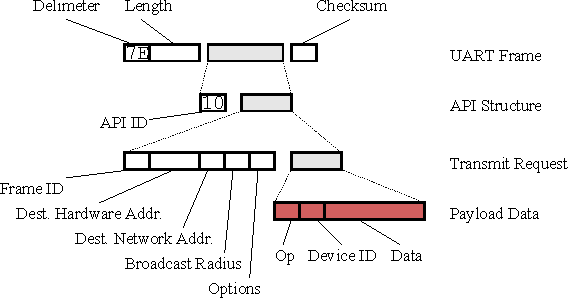
\includegraphics[width=\textwidth]{images/packets.pdf}
\caption{Composition of an example ZigBee API frame transmitted via the UART}
\label{packets-example}
\end{figure}

Besides the data payload described above, the command frames contain a lot of extra information required for parsing the structure. A delimeter marks the beginning of the packet, then two length bytes give the size of the API structure, and a checksum is used for error detection. The API ID specifies the type of frame that is being sent, in this case (\texttt{0x10}) it is a Zigbee Transmit Request frame that includes different target addresses (with special values being used to address the coordinator or broadcast mode). Following these, and a number of extra options that are not used in the context of the project, is the final payload data.

\section{Transport Layer}
The transport layer provides an interface to the serial link (in these implementations, using the UART peripheral of the ARM processors) used to communicate with the ZigBee nodes. This is the main differentiating factor between the master and scale units.

\subsection{Exposed Transport API}
The interface used by higher layers is exposed through \texttt{zb\_transport.h}. It is modelled as a subset of the most basic network operations, only implementing those required by the system -- that is, reading data as individual characters for passing them to the packet layer parser, and writing data as blocks of multiple bytes, for sending complete packets.

First of all, the system must be initialised using \texttt{zb\_transport\_init()}. Then data can be received character by character, in the order received, through the blocking \texttt{zb\_getc()} call. Finally, data can be sent to the device by providing an array of bytes and its size to \texttt{zb\_send()}. The \texttt{zb\_transport\_stop()} method has been added to perform clean-up operations such as closing file handles or freeing dynamically allocated structures on implementations that require it.

\subsection{Linux Implementation}
The Raspberry Pi runs a complete Linux distribution, and the microprocessor's UART peripheral is exposed as a serial port to the system, found in \texttt{/dev/ttyAMA0}. This port can be accessed using standard file operation system calls such as \texttt{read} and \texttt{write} after having been initialised by opening the file and setting a number of standard serial options \cite{posix-serial-programming}. Outside of this software implementation, the system must be configured to not send kernel debug messages to the port\cite{pi-tty}.

A separate thread (implemented using the pthread library \cite{pthread}) is running in the background, continuously monitoring the serial port by blocking on \texttt{read()}. When a character is received on the serial port, it gets stored in a thread safe bounded buffer structure from which characters can later be  retrieved by a higher layer implementation. Thread safety is ensured by using pthread condition variables and locks.

\subsection{Microcontroller Implementation}
On the microcontroller, no threading capabilities besides raw interrupts are available by default, and the serial link is implemented as a peripheral component of the microcontroller. ST provides driver libraries for configuring and accessing such peripherals which have been used extensively for this implementation. Further operating systems such as TinyOS, Kontiki, or InceOS were not initially considered as the team only became aware of their existence well into the implementation phase. However, due to the very simple functionality required of the scale units, their inclusion would likely have made the system more extensible at the cost of complication for the initial implementation.

The UART peripheral provides a small hardware buffer that is currently used as the only buffer in this implementation due to the low frequency of packets and relatively short non-IO bursts in the software. Therefore, the \texttt{zb\_getc} implementation is currently busy-waiting for the memory-mapped UART status register to clear its \emph{RXNE} (Receive buffer non-empty) flag. This is a similiar structure to waiting for a condition variable in a pthread program. %TODO check if we can actually wait for interrupts here to put the processor to sleep, saving power and getting rid of bad busy waiting. Yes we could, but it still wouldn't help the receive-while-sending race condition.

This polling method uses busy waiting, and is therefore is inherently using more power by keeping the processor busy in a loop all the time. It is also less flexible than waiting for interrupts. However, for prototyping and debugging, this made the implementation and testing much easier. It is expected that this part of the system can be re-developed using interrupts and additional software buffering should multi-tasking be required in the future, e.g. if more complicated processing (thus tightening the time constraints) is required.

Since the serial data rate for the ZigBee units (in default configuration) is 9600 baud, and the clock speed of the microcontroller is 168MHz, there is more than enough time to complete any required processing inbetween receiving two characters.

%TODO MATH.

A flaw in the current design is that no data can be received if it is sent while the unit is currently also sending data. This case should be rare, and did not occur during testing, but may still be possible. It should not cause complete system failure, but the packet to be received will be lost and needs to be retransmitted completely by the other end's transport layer, which can currently only be achieved by the application requesting the same packet to be sent again. Retransmission by the ZigBee layer does not solve the issue, as the RF ACK will have been sent, but there is currently no dedicated acknowledgement of UART frames, though this is supported by the ZigBee devices. %TODO reword this - does it make sense?

\section{Packet Layer}
The packet layer provides an abstraction for sending and receiving custom data in a fixed format using the transport layer. Its implementation is identical for all units, the only changes required are in the application layer's initialisation calls.

The first implementation, which was used for testing the transport layer due its simplicity, was based on a custom packet format that had nothing more than the aforementioned data content, a delimeter, and a checksum. The ZigBee units were pre-configured with destination addresses and options, and used in transparent mode.

Due to the issues explained in \ref{section:software-impl-packets}, transparent mode had to be dropped and a second packet layer implementation tailored to the ZigBee API mode was developed using the same API calls. This is described in the following sections. 

\subsection{Packet API}
The public API for the packet layer is defined in \texttt{zb\_packets.h}. 

Initialisation and settings are provided through the \texttt{zb\_packets\_init}, \texttt{zb\_set\_broadcast\_mode}, and \texttt{zb\_set\_device\_id} methods. In the current implementation, broadcast mode is the only way to set the target address: The master unit sends broadcast packages that are received by all scale units, and the scale units send unicast packages targeted only at the master unit. This state is held in a global variable, and it would be trivial to add functionality to support arbitrary target addresses, though this would require for the application layer to know about network or device addresses of the destination.

%TODO missing abstraction: Stop/close/destroy call should be to packets layer and handed down to transport.

\subsection{Parsing Methodology}
The ZigBee API defines data frames transmitted across the serial link between the host and ZigBee device. These packets are parsed and, if the packet is a transmission request, wrapped in a different 802.15.4 packet for transmission over the air, and re-packaged in a serial data frame by the receiving device. The relevant API frames for this design are ''Zigbee Transmit Request'', ``ZigBee Transmission Received'', and ``AT Command Request'' \cite[cf. section 6, API Operation]{xbee-datasheet}.

Re-Transmission if checksums fail or no ACKs are received for these over-the-air packets is handled at the ZigBee layer that is equivalent to the Network layer in the OSI model (\textbf{TODO confirm and cite this}), and in this implementation is completely independent from even the application transport layer.

Parsing of the incoming character stream is achieved through the \texttt{zb\_parse} method which must be called on every character received. It returns a status code to indicate when a complete packet has been received. At this point, globally available variables are filled with the relevant information (op code, device id, data, length) from the packet. The method is implemented as a finite state machine with the state maintained in static local variables. This implementation is inspired by the Yacc parser/lexer architecture\cite{yacc}. In retrospect, these tools could well have been used for the implementation. Due to time constraints in the development phase, and initially starting off with a considerably smaller parser for the simpler packet structure, this was not fully considered before most of the implementation was completed. 

\section{Application Layer}

\begin{figure}
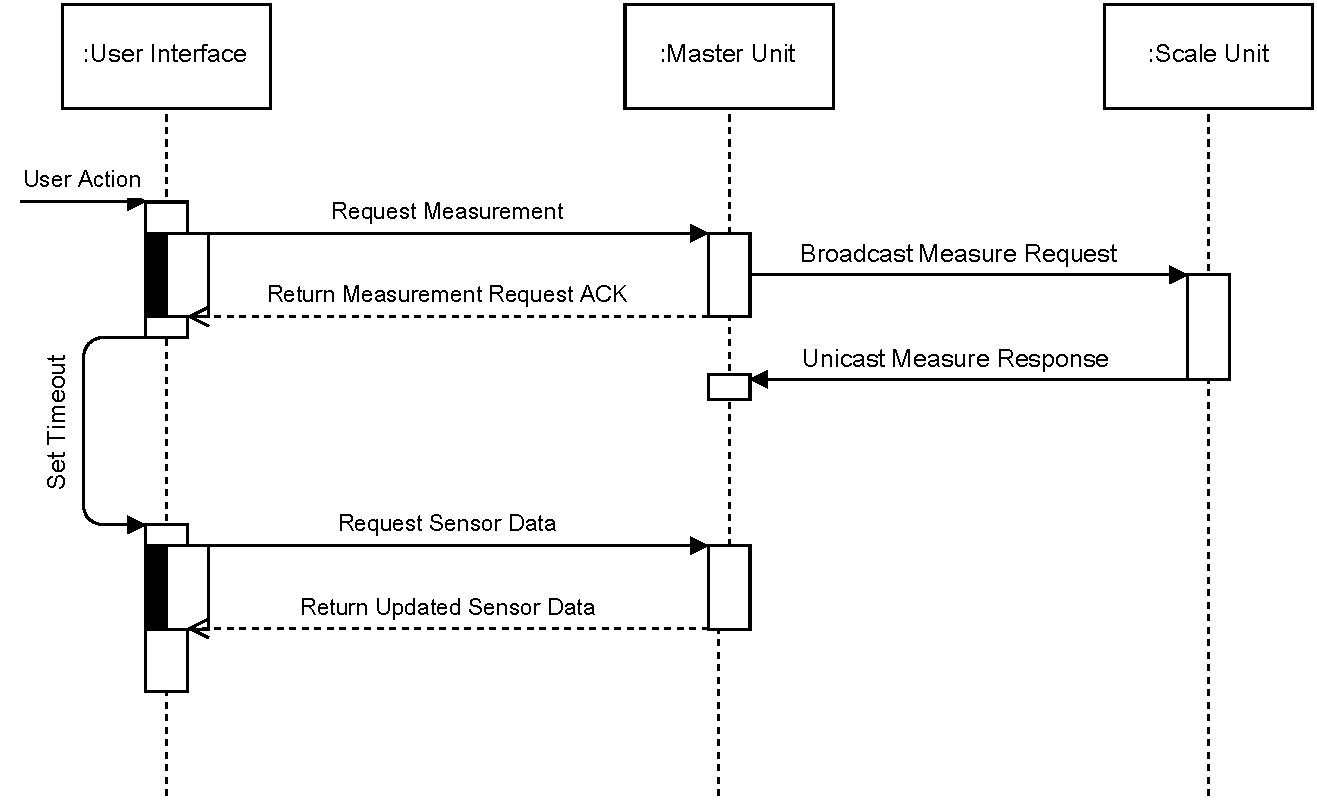
\includegraphics[width=\textwidth]{images/communications-diagram.pdf}
\caption{Application Level Communications Diagram}
\label{communications-diagram}
\end{figure}

Figure \ref{communications-diagram} shows the interaction between the various devices for servicing a user request for updating the measurements. Note that the shown units are entire programs running on different devices, rather than individual threads of control within a single program. One scale unit is shown exemplary. When multiple scale units are used, and all try to respond to the broadcast measure request, their packets are linearised by the receiving ZigBee coordinator.

\subsection{Master Unit}
The master unit program is integrated with a web-server, which is single-threaded to keep the implementation as simple as possible. Since the system will only be used by one or two clients simultaneously, a high-performance implementation is not required as this point. A thread seperate to the webserver uses the packet layer to scan for incoming RF packets and update the thread-safe sensor results data structure with new values as they come in.

Request handlers, which are called when an HTTP request matches an API call path, have been abstracted out into \texttt{requesthandlers.c} so that they can also be invoked manually in the master\_test command-line application. This file manages all state associated with sensors: Their last update time and value, settings such as the calibration offset, as well as a global indicator of when the last RF message was sent. This value is used to provide a primitive time-out mechanism to prevent overloading the serial and RF links if many measure requests come in simultaneously, either due to a bug in the client application or malicious intent. Within one second of the last measurement request, all new incoming measurement or calibration requests are ignored, and an error message is sent to the requesting client.

For serving the user interface, a version of the webserver produced for previous coursework\cite{ns3-coursework} has been used. It was considered to integrate the master unit code with a larger open source software package such as Apache \cite{apache}, possibly as an add-on module. Alternatively, an interface between the request handler C methods and another programming language with existing web-server libraries such as Python could have been developed. However, for prototyping, the decision was made to keep things as simple as possible, and as only a limited amount of time was available, this approach that was already well understood by the team was taken.

The conversion from sensor value to weight is performed on the server. Similarly, the calibration method is implemented by storing an offset for each sensor on the master unit, which is updated with the current sensor readings when the user requests a calibration. As a placeholder for actual calibration and conversion functionality, the conversion is performed by dividing by a constant, where the calibration is just a fixed offset. It is expected that the methods for conversion and calibration will need to be significantly more complicated, as the strain gauge's change in resistance, and thus ADC input voltage, does not scale linearly with weight but can be approximated with \textbf{ASK JOSH WHAT MATHEMATICAL FUCNTION REPERSNTS THIS}.

\subsection{Scale Unit}
The scale unit software has been kept very minimal. The same packet layer implementation written for the master unit is re-used here. The program consists of a single infinite loop that retrieves characters from the UART using the transport layer, calls the parser, and sends a response if a complete valid packet has been retrieved. The response data is read from the Analogue-to-Digital converter (ADC) that is connected to the strain gauge instrumentation amplifier.

The ADC peripheral has been configured in continous conversion DMA (direct memory access) mode. This means that the conversions are handled purely by hardware, and the results can be accessed through a global variable at any time with no additional delay or processing. The conversion rate for this is \textbf{CONVERSION RATE FOR DMA MODE ADC AND SOURCE FOR THIS}.


\subsection{User Interface}
The user interface to the system has been defined \ref{section:requirements} to be a very simple web application that should support taking readings of the current system state by intitiating measurements, as well as providing simple calibration of the scales. A mock-up was drawn up, and based on this a static HTML/CSS prototype was generated. This was then made interactive by attaching Javascript actions to the buttons.

The client side (running in the user's web-browser) logic is implemented using the jQuery Javascript framework \cite{jquery} which provides simple abstractions for modifying the displayed documents (switching between sections and responding to user events such as button clicks), sending asynchronous HTTP requests, and parsing responses to them. This is used to make calls to special paths that are mapped to methods initiating data transfers between the master and scale units, or returning data previously stored on the server:

\begin{itemize}
	\item \texttt{/api/data} returns a JSON \cite{json-spec} object containing the data stored on the master unit for all sensors (raw value, converted value, last response time).
	\item \texttt{/api/calibrate} initiates a measurement on all scale units and sets the values received to be the zero-points for that particular sensor.
	\item \texttt{/api/measure} initiates a measurement and stores the results in a server-side structure to be later retreived by a \texttt{data} request.
\end{itemize}

\begin{figure}
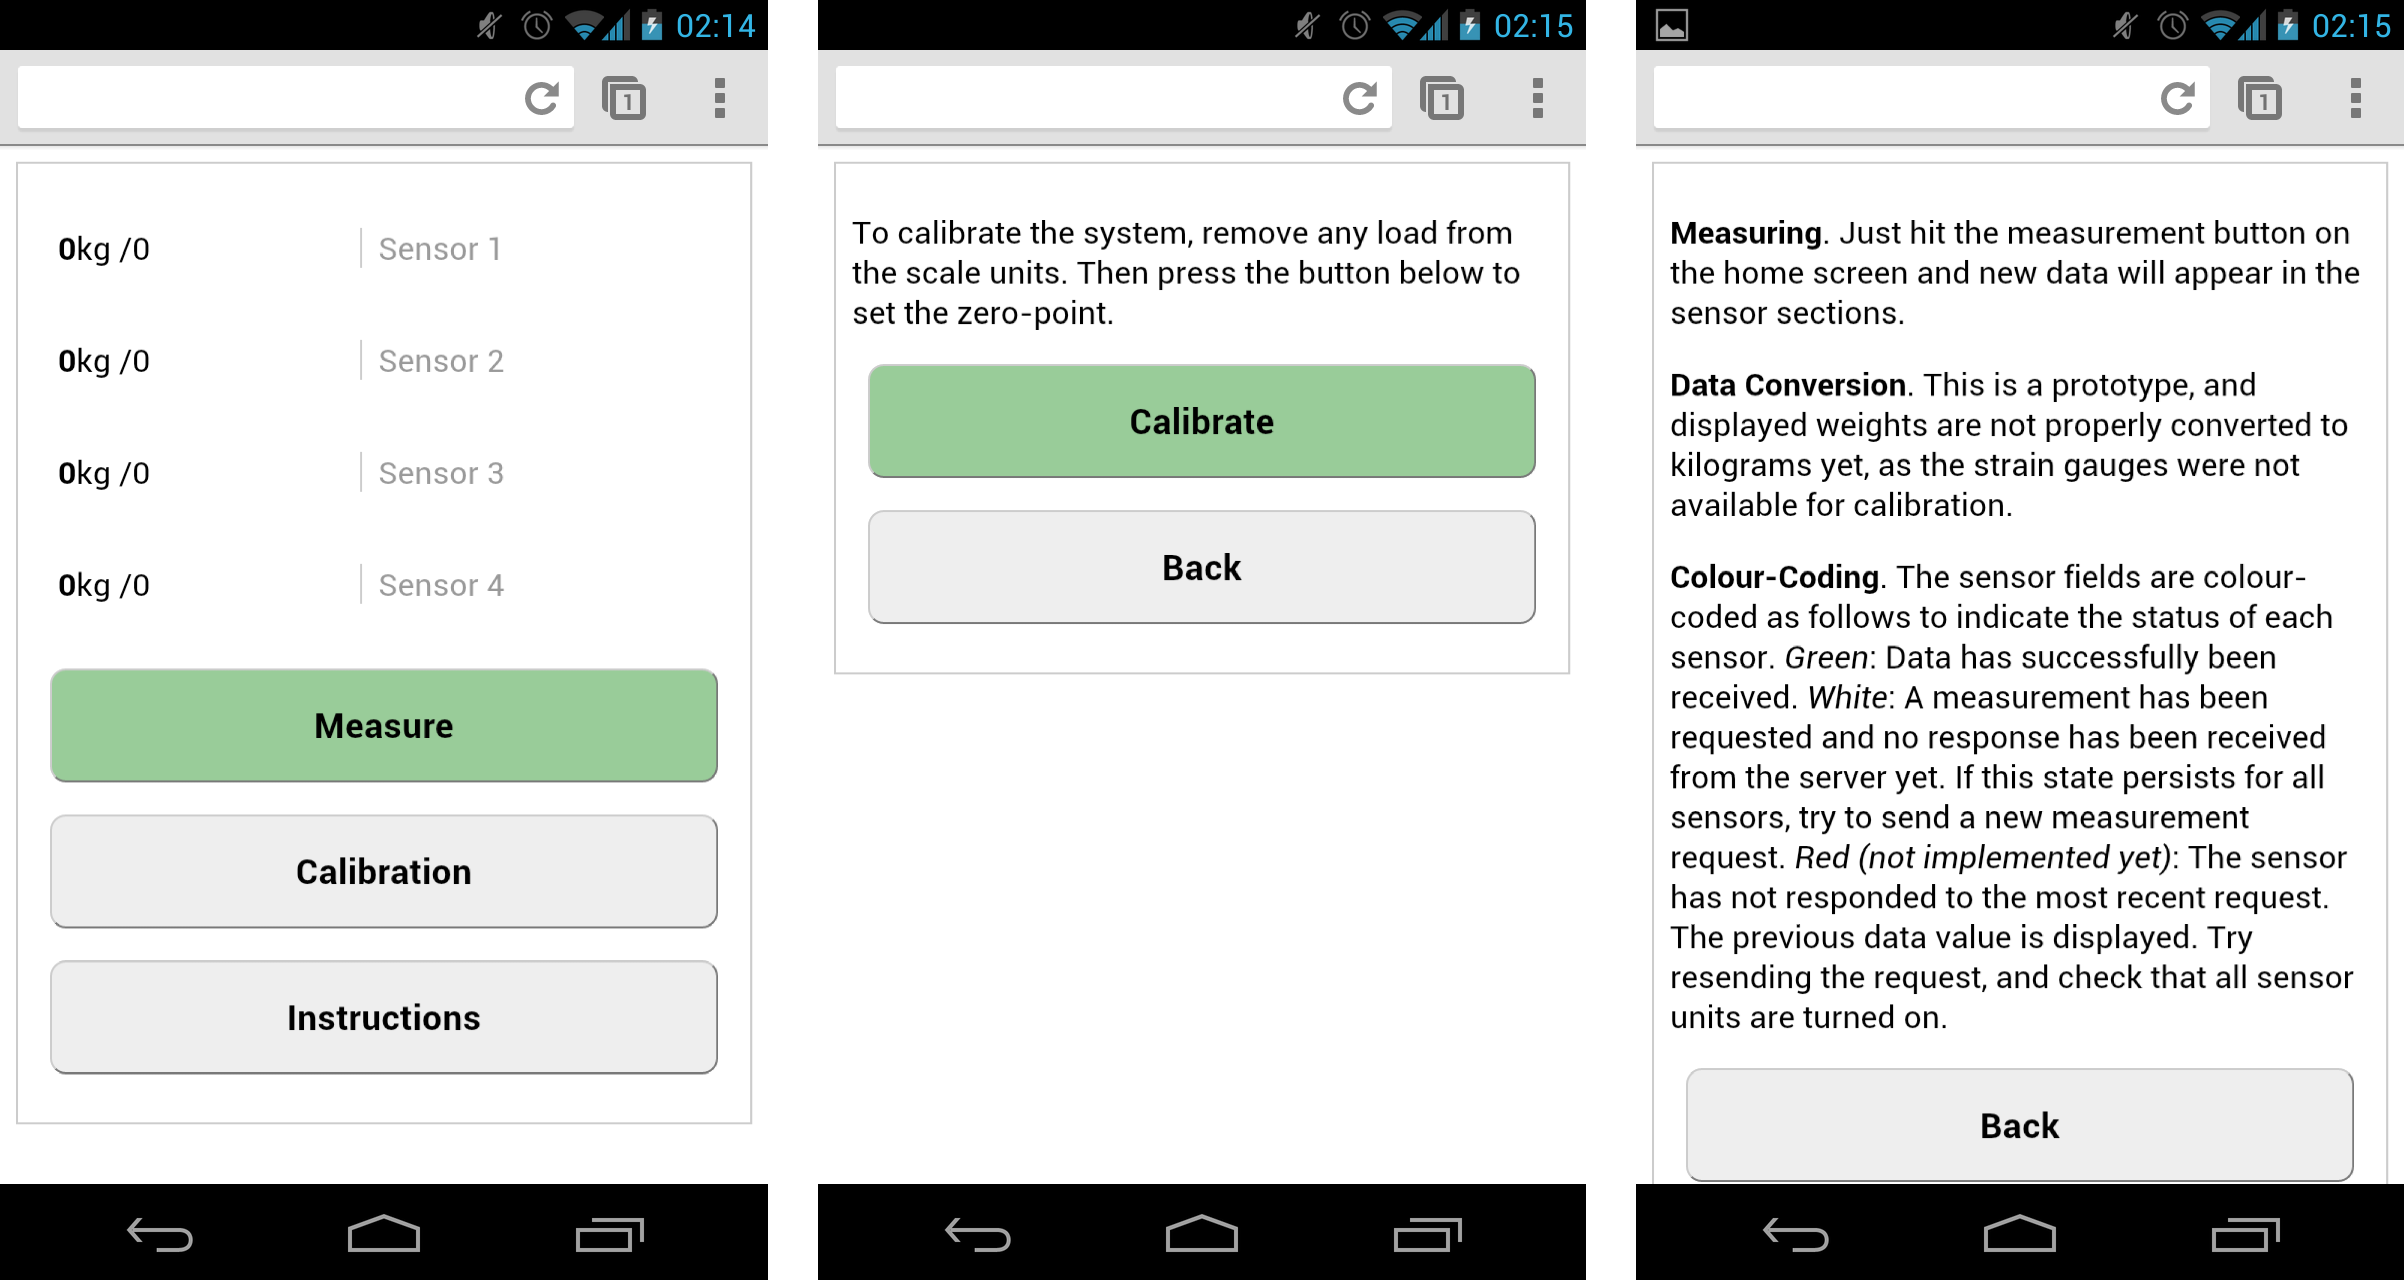
\includegraphics[width=\textwidth]{images/screenshots/ui-screenshot.png}
\caption{User Interface Screens, viewed on an Android phone within the Chrome browser}
\label{ui-screenshot}
\end{figure}

The design was informed by the main target platform which are small touch screens on smart phones (e.g. Android or iOS), or tablets. Therefore, the number of buttons has been kept as low as possible, and the main focus is on displaying crucial information. Colour-coding the background of each sensor section is used to provide visual feedback to user interface actions and system status, to avoid using up more screen real-estate. A quick start guide is included through the ``Instructions'' button. Since calibration can have a very confusing effect if there is still some weights on the scales when it is initiated, this has been made into a two-step process: The user has to open the calibration screen and confirm the action, a helpful note about the effects is displayed with the confirmation button.

Of course, this design leaves room for expansion. For example, one could envision a slider component to view previously retrieved measurements, as well as different display modes to do some data analysis on the raw values received, such as displaying differential weights for the left/right and front/rear distribution. Before final delivery of the system, the scale units must be marked with labels to indicate which wheel they are meant for, and then the ``Sensor n'' labels can be replaced with ``front-left'', and so on.
